\documentclass[border=0.8ex,svgnames,tikz]{standalone}
\usepackage{amsmath,mathtools}
\usepackage{fontspec}
\setmainfont{Source Serif 4}
\setsansfont{Source Sans 3}
\setmonofont{Source Code Pro}
\usetikzlibrary{positioning,chains}
\newcommand{\ptrcolor}{LightSlateBlue}
\newcommand{\itcolor}{IndianRed}
\newcommand{\ritcolor}{LimeGreen}
\begin{document}
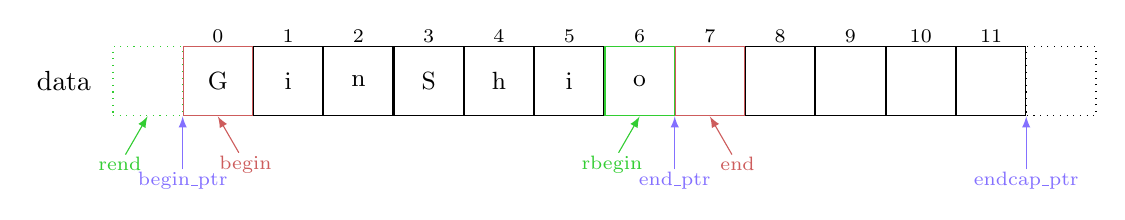
\begin{tikzpicture}
  \begin{scope}[
    node distance=0,
    every node/.style={draw,on chain,inner sep=1ex,minimum width=2.5em,minimum
      height=2.5em,font=\small},
    index node/.style={draw=none,on chain,inner sep=0ex,minimum
      width=2.5em,minimum height=1.5ex,font=\scriptsize},
    start chain=going right,
    ]
    % datas
    \node[dotted,draw=\ritcolor](rend){};
    \node[draw=\itcolor](begin){G};
    \node{i};
    \node{n};
    \node{S};
    \node{h};
    \node{i};
    \node[draw=\ritcolor](rbegin){o};
    \node[draw=\itcolor](end){};
    \node{};
    \node{};
    \node{};
    \node{};
    \node[dotted](endcap){};
    % indices
    \node[index node,above=of rend]{};
    \node[index node]{0};
    \node[index node]{1};
    \node[index node]{2};
    \node[index node]{3};
    \node[index node]{4};
    \node[index node]{5};
    \node[index node]{6};
    \node[index node]{7};
    \node[index node]{8};
    \node[index node]{9};
    \node[index node]{10};
    \node[index node]{11};
  \end{scope}
  \begin{scope}[
    every path/.style={draw,>=latex},
    every node/.style={draw=none,inner sep=0.2ex,font=\scriptsize},
    ]
    \path[color=\ptrcolor,text=\ptrcolor]
    (begin.west) ++(0,-3.6em) node{begin\_ptr} edge[->] (begin.south west)
    (end.west) ++(0,-3.6em) node{end\_ptr} edge[->] (end.south west)
    (endcap.west) ++(0,-3.6em) node{endcap\_ptr} edge[->] (endcap.south west);
    \path[color=\itcolor,text=\itcolor]
    (begin) ++(1.0em,-3em) node{begin} edge[->] (begin.south)
    (end) ++(1.0em,-3em) node{end} edge[->] (end.south);
    \path[color=\ritcolor,text=\ritcolor]
    (rend) ++(-1.0em,-3em) node{rend} edge[->] (rend.south)
    (rbegin) ++(-1.0em,-3em) node{rbegin} edge[->] (rbegin.south);
  \end{scope}
  \node[left=1ex of rend]{data};
\end{tikzpicture}
\end{document}
